
% This LaTeX was auto-generated from MATLAB code.
% To make changes, update the MATLAB code and republish this document.

\documentclass{article}
\usepackage[section]{placeins}
\usepackage{graphicx}
\usepackage{color}
\usepackage{multirow}
\usepackage{float}
\sloppy
\definecolor{lightgray}{gray}{0.5}

\newcommand\tab[1][1cm]{\hspace*{#1}}
\begin{document}

\section{Introduction}

The data were collected at four different speed on the treadmill from speed 1 to 4. Each speed is collected twice at 20 steps, one for training data and one for test dataset.

The stride detection algorithm is simply find the peaks that is above certain threshold with a certain minimum time intervals. The features that are selected are peaks, troughs, period.

\section{X Axis}

The following shows the mean, root mean square, standard deviation for all four different speeds as well as the mean peaks and troughs values.

\begin{verbatim}Speed 1:
     Mean :-1.115
     RMS  :1.133
     STD  :0.200
     Mean Min :0.389
     Mean Max :0.592
Speed 2:
     Mean :-1.173
     RMS  :1.225
     STD  :0.353
     Mean Min :0.798
     Mean Max :1.015
Speed 3:
     Mean :-1.291
     RMS  :1.433
     STD  :0.622
     Mean Min :1.723
     Mean Max :1.345
Speed 4:
     Mean :-1.419
     RMS  :1.602
     STD  :0.743
     Mean Min :1.678
     Mean Max :1.603
\end{verbatim} 
    
For x axis, the root mean square, standard deviation and mean max value are significantly different with the trend that all of them go up when the speed goes up.

The following figures show the peaks and troughs detected for all four speeds for x axis.

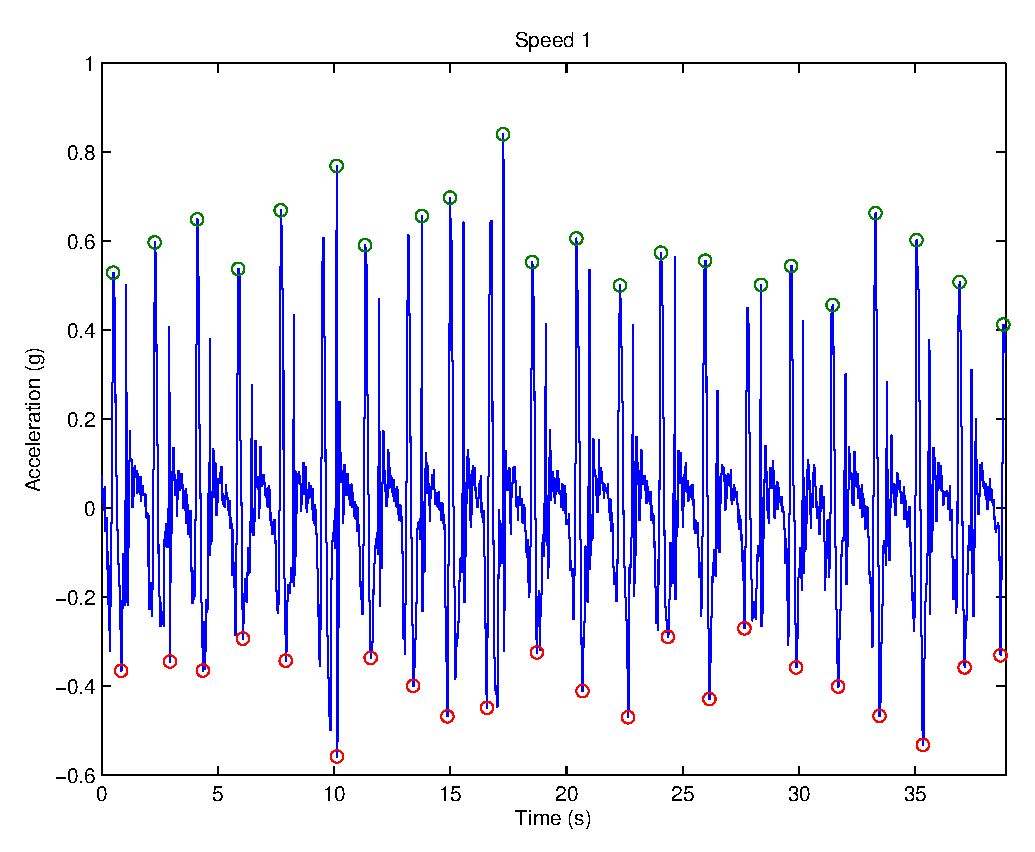
\includegraphics [width=4in]{printout_01.eps}

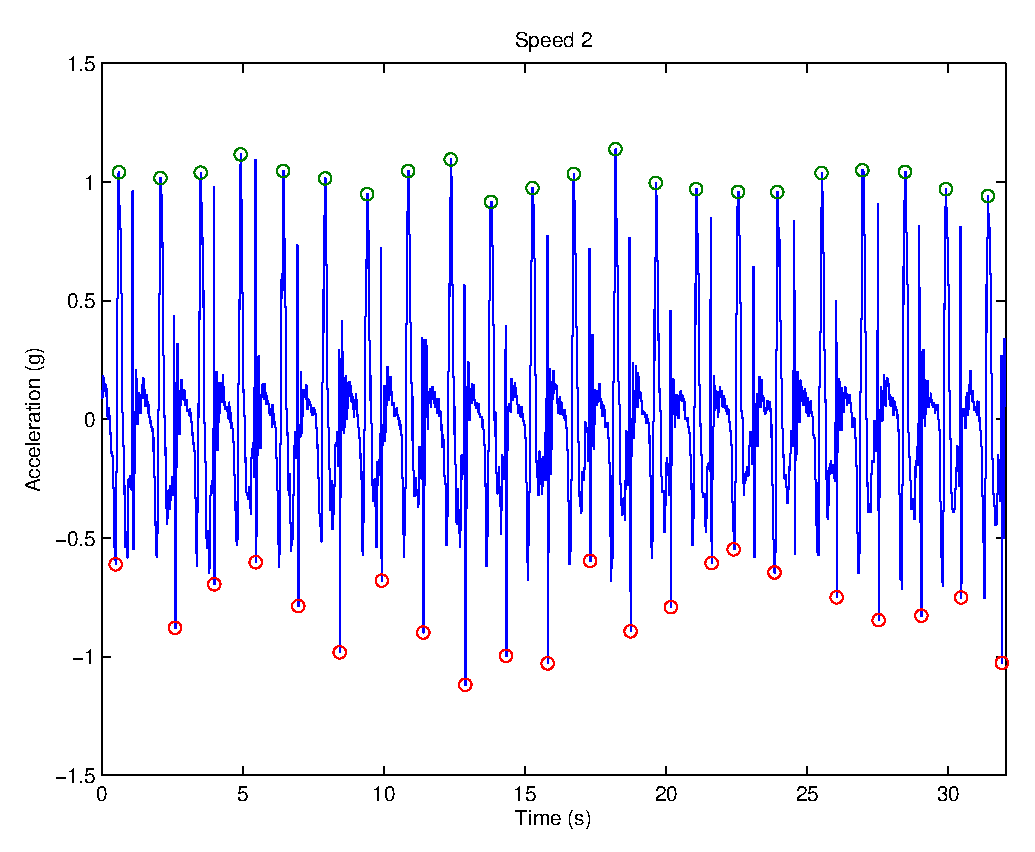
\includegraphics [width=4in]{printout_02.eps}

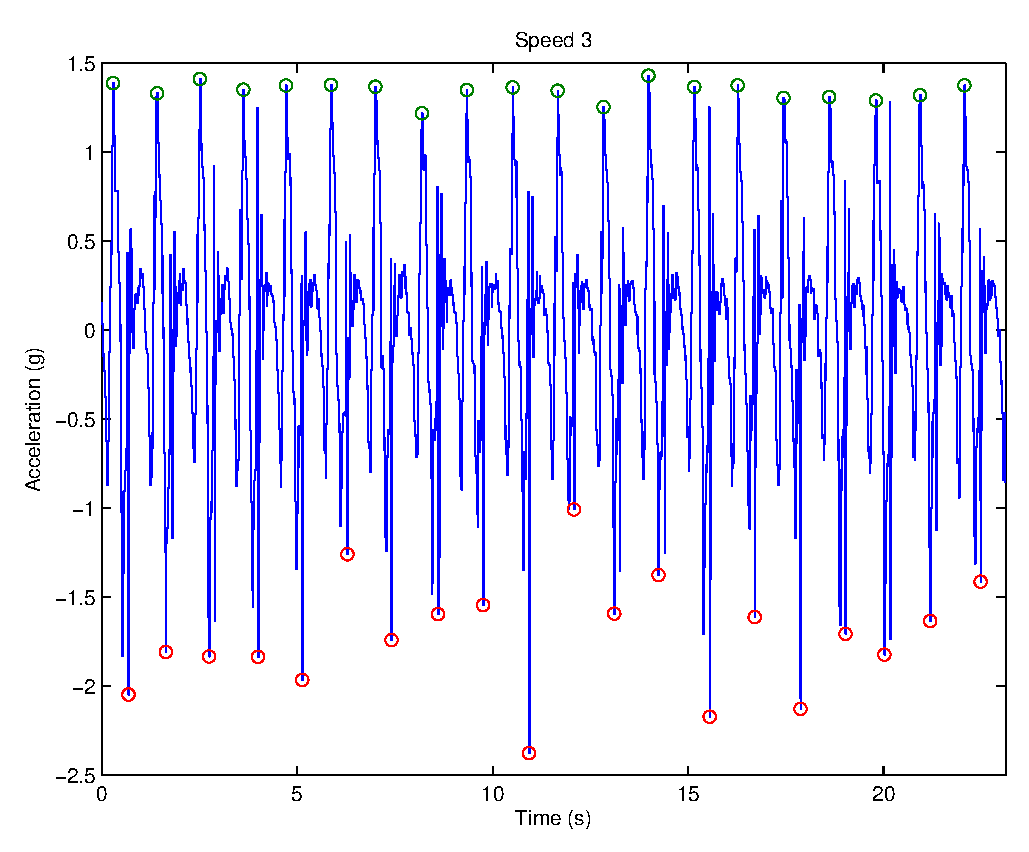
\includegraphics [width=4in]{printout_03.eps}

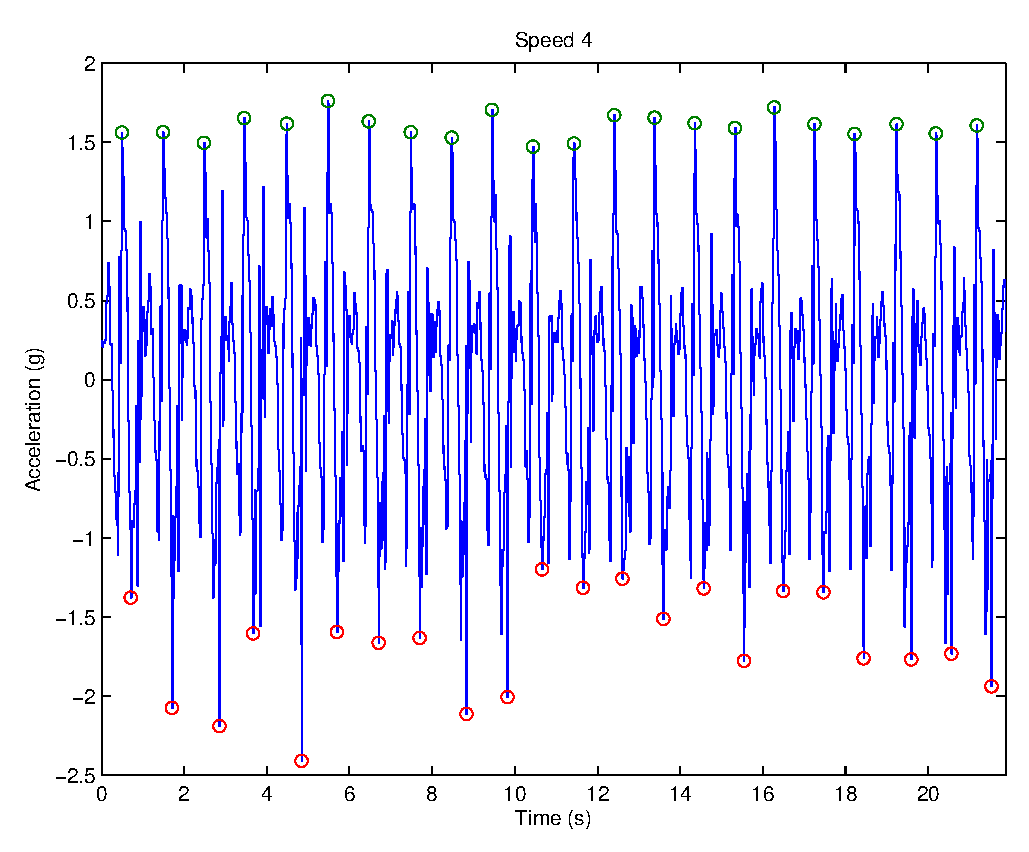
\includegraphics [width=4in]{printout_04.eps}

\begin{table}[H]
\centering
\caption{Confusion Matrix}
\label{my-label}
\begin{tabular}{cc|c|c|c|c}
\hline
                                             &         & \multicolumn{4}{c}{Predicted}        \\ \cline{3-6} 
                                             &         & Speed 1 & Speed 2 & Speed 3 & Speed 4 \\ \hline
\multicolumn{1}{c|}{\multirow{4}{*}{Actual}} & Speed 1 & 19      & 2       & 0       & 0       \\
\multicolumn{1}{c|}{}                        & Speed 2 & 0       & 21      & 0       & 0       \\
\multicolumn{1}{c|}{}                        & Speed 3 & 0       & 1       & 18      & 0       \\
\multicolumn{1}{c|}{}                        & Speed 4 & 0       & 0       & 0       & 21      \\ \hline
\end{tabular}
\end{table}
\section{Y Axis}


The following shows the mean, root mean square, standard deviation for all four different speeds as well as the mean peaks and troughs values.

\begin{verbatim}Speed 1:
     Mean :0.029
     RMS  :0.247
     STD  :0.245
     Mean Min :0.494
     Mean Max :1.355
Speed 2:
     Mean :-0.031
     RMS  :0.442
     STD  :0.441
     Mean Min :0.921
     Mean Max :2.595
Speed 3:
     Mean :-0.053
     RMS  :0.758
     STD  :0.756
     Mean Min :2.089
     Mean Max :3.261
Speed 4:
     Mean :-0.095
     RMS  :1.019
     STD  :1.014
     Mean Min :2.822
     Mean Max :2.814
\end{verbatim} 

For y axis, the mean, root mean square, standard deviation and mean min value are significantly different with the trend that all of them go up when the speed goes up.

The following figures show the peaks and troughs detected for all four speeds for y axis.

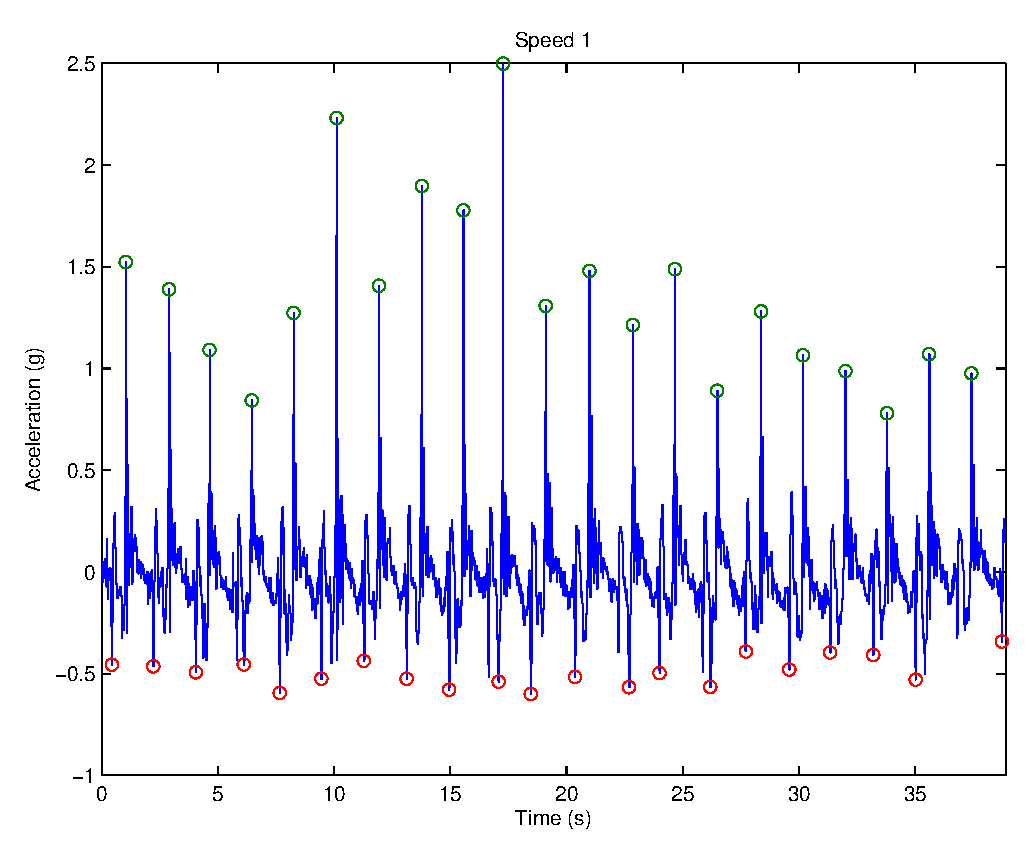
\includegraphics [width=4in]{printout_05.eps}

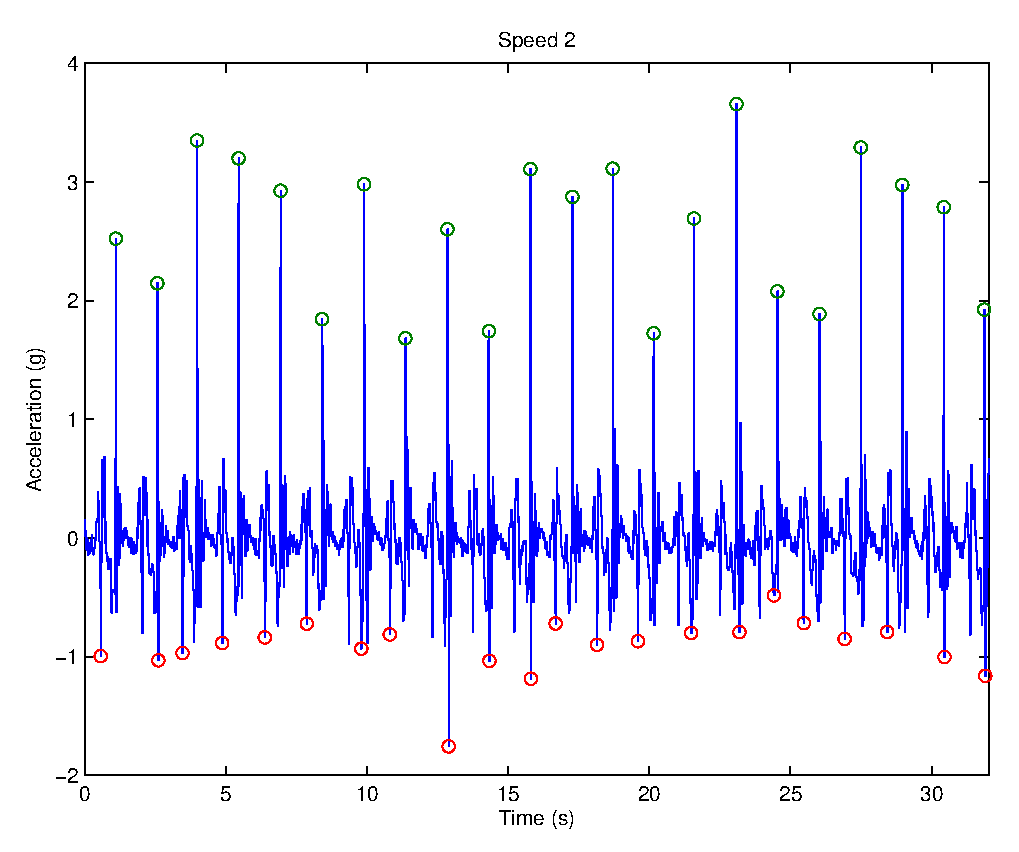
\includegraphics [width=4in]{printout_06.eps}

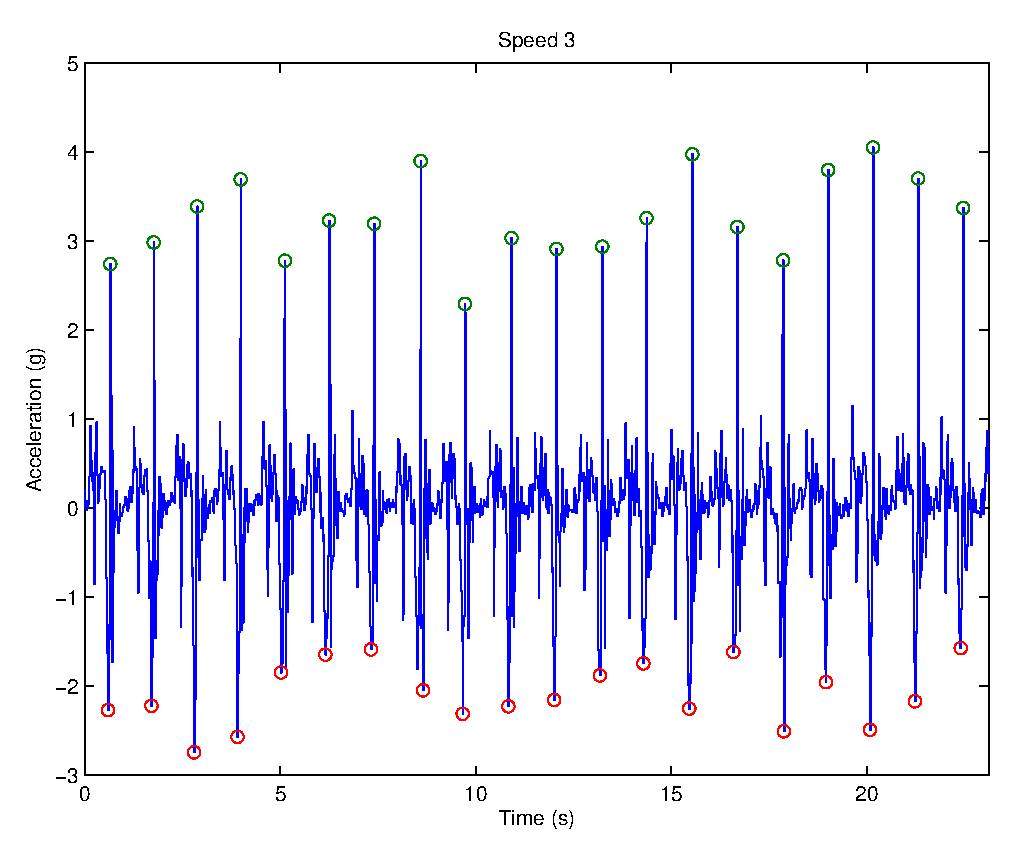
\includegraphics [width=4in]{printout_07.eps}

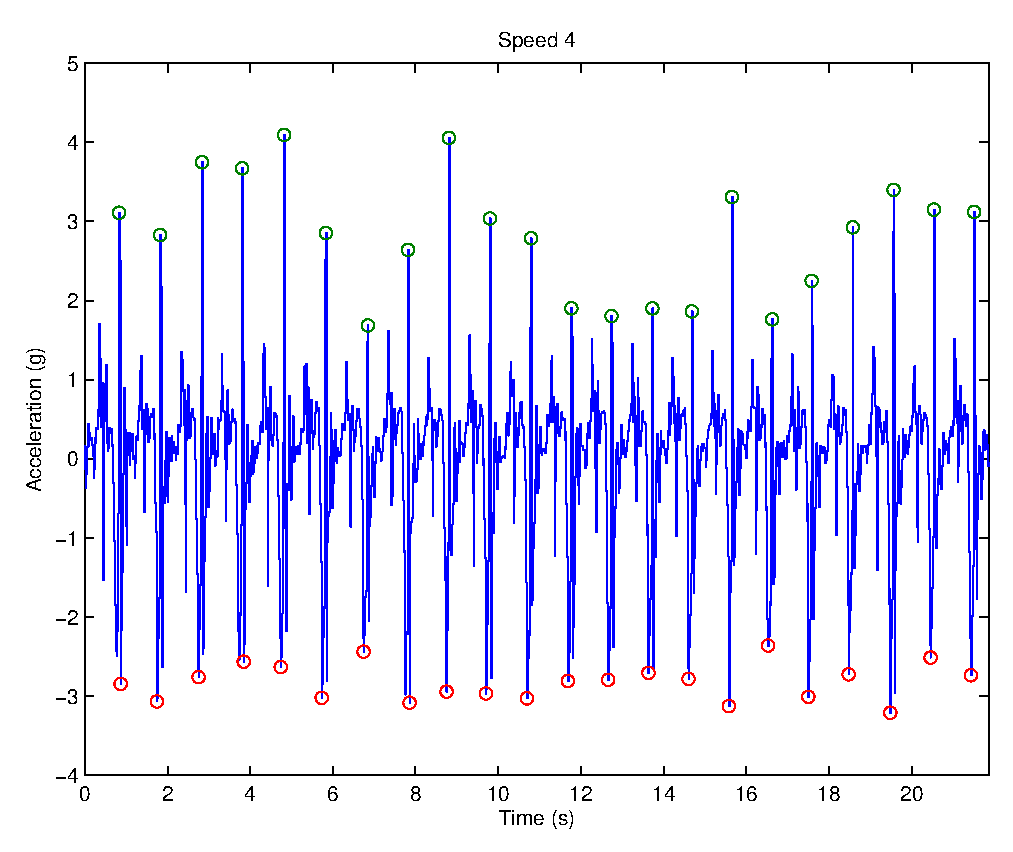
\includegraphics [width=4in]{printout_08.eps}

% Please add the following required packages to your document preamble:
% \usepackage{multirow}
\begin{table}[H]
\centering
\caption{Confusion Matrix}
\begin{tabular}{cc|c|c|c|c}
\hline
                                             &         & \multicolumn{4}{c}{Predicted}        \\ \cline{3-6} 
                                             &         & Speed 1 & Speed 2 & Speed 3 & Speed 4 \\ \hline
\multicolumn{1}{c|}{\multirow{4}{*}{Actual}} & Speed 1 & 19      & 1       & 0       & 0       \\
\multicolumn{1}{c|}{}                        & Speed 2 & 0       & 20      & 1       & 0       \\
\multicolumn{1}{c|}{}                        & Speed 3 & 0       & 0       & 18      & 1       \\
\multicolumn{1}{c|}{}                        & Speed 4 & 0       & 0       & 1       & 20      \\ \hline
\end{tabular}
\end{table}

\section{Z Axis}



The following shows the mean, root mean square, standard deviation for all four different speeds as well as the mean peaks and troughs values.

\begin{verbatim}Speed 1:
     Mean :-0.291
     RMS  :0.324
     STD  :0.143
     Mean Min :0.557
     Mean Max :0.309
Speed 2:
     Mean :-0.284
     RMS  :0.366
     STD  :0.231
     Mean Min :0.870
     Mean Max :0.722
Speed 3:
     Mean :-0.340
     RMS  :0.538
     STD  :0.416
     Mean Min :1.226
     Mean Max :1.564
Speed 4:
     Mean :-0.422
     RMS  :0.709
     STD  :0.570
     Mean Min :1.457
     Mean Max :1.588
\end{verbatim} 
    
    For y axis, the root mean square, standard deviation and mean min value are significantly different with the trend that all of them go up when the speed goes up.
    
    The following figures show the peaks and troughs detected for all four speeds for z axis.
    
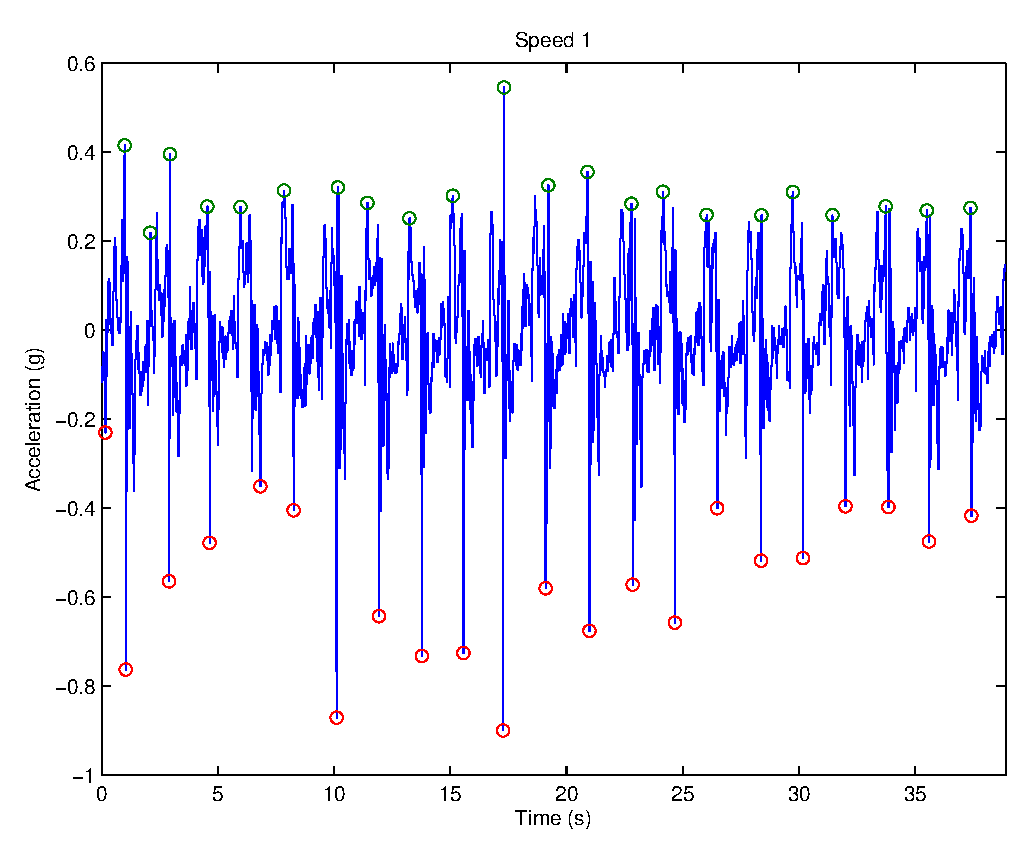
\includegraphics [width=4in]{printout_09.eps}

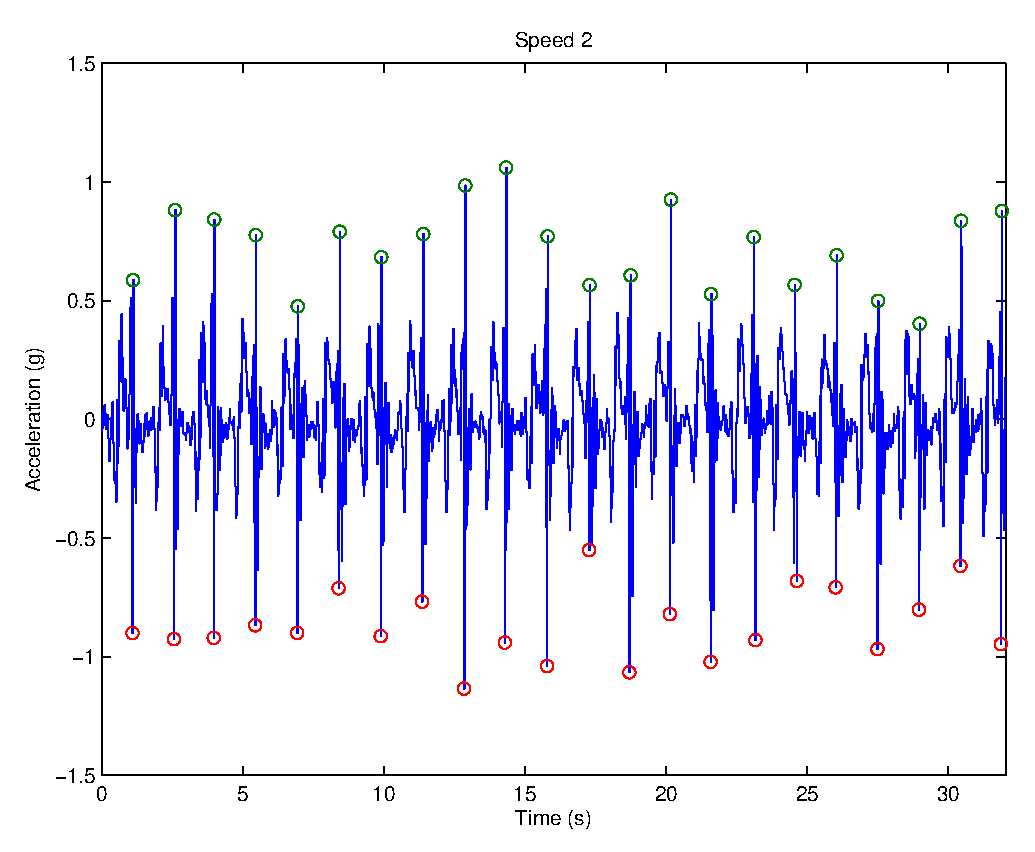
\includegraphics [width=4in]{printout_10.eps}

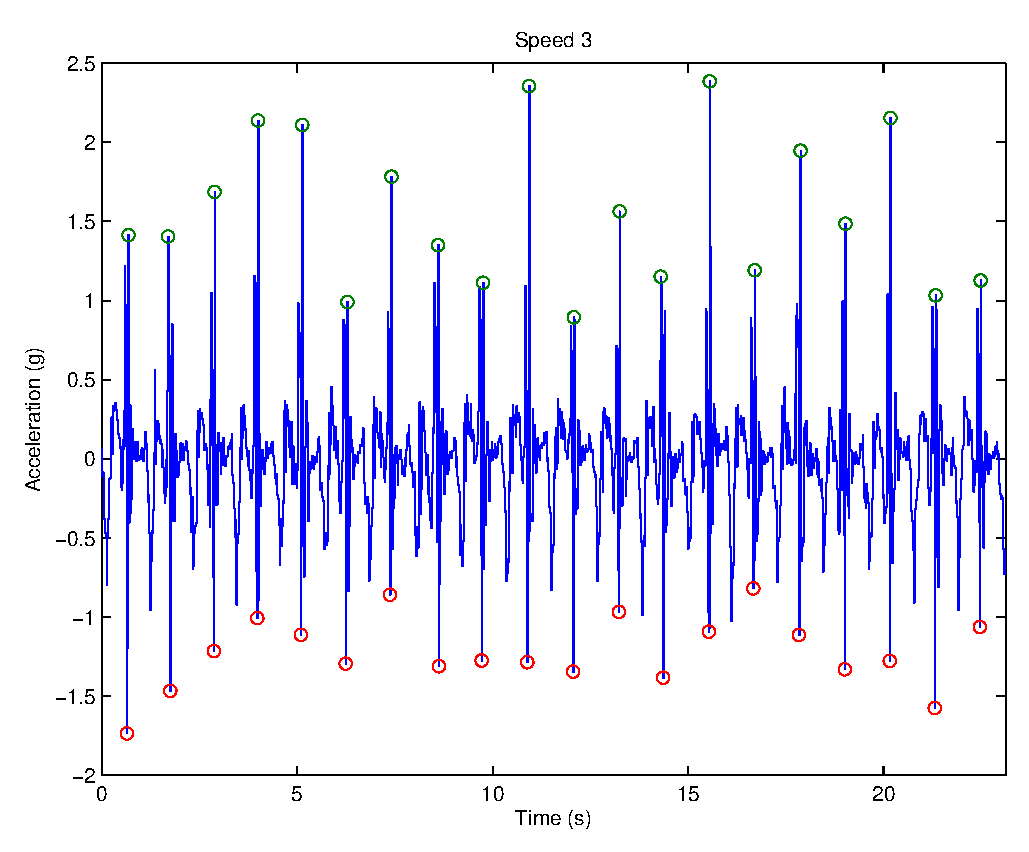
\includegraphics [width=4in]{printout_11.eps}

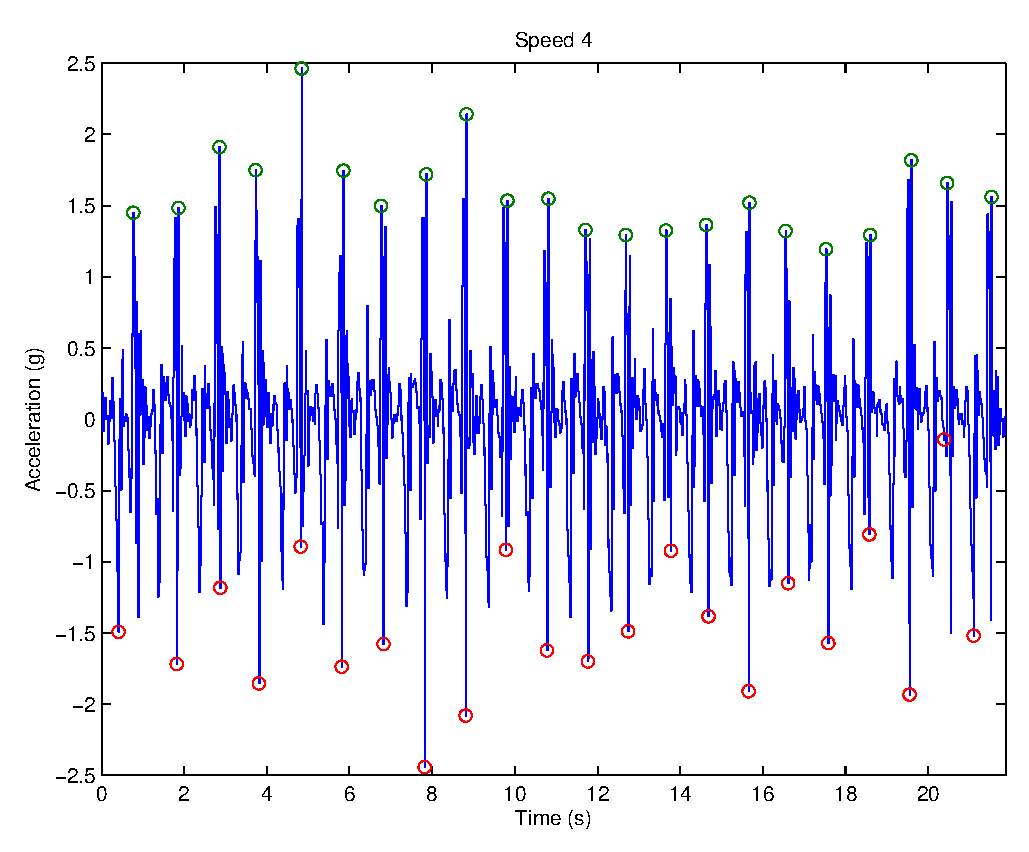
\includegraphics [width=4in]{printout_12.eps}

% Please add the following required packages to your document preamble:
% \usepackage{multirow}
\begin{table}[H]
\centering
\caption{Confusion Matrix}
\begin{tabular}{cc|c|c|c|c}
\hline
                                             &         & \multicolumn{4}{c}{Predicted}        \\ \cline{3-6} 
                                             &         & Speed 1 & Speed 2 & Speed 3 & Speed 4 \\ \hline
\multicolumn{1}{c|}{\multirow{4}{*}{Actual}} & Speed 1 & 17      & 2       & 1       & 1       \\
\multicolumn{1}{c|}{}                        & Speed 2 & 0       & 20      & 1       & 0       \\
\multicolumn{1}{c|}{}                        & Speed 3 & 0       & 0       & 16      & 3       \\
\multicolumn{1}{c|}{}                        & Speed 4 & 0       & 0       & 4       & 17      \\ \hline
\end{tabular}
\end{table}

\section{Discussion}

From all three confusion matrices, it is easily to realize that both x and y axis are able to classified the test data set based on the train data set. Yet, for z axis, more misclassifications show up. This can be explained by the peaks and troughs shape. Since for x and y axis, the peaks and trough for one speed looks alike, especially the amplitudes between each peak and trough. However, for z axis, this is not true which could be harder for neural network to classify.
\end{document}
    
